\documentclass{article}
\usepackage[final]{nips_2017}
\usepackage[utf8]{inputenc} % allow utf-8 input
\usepackage[T1]{fontenc}    % use 8-bit T1 fonts
\usepackage{hyperref}       % hyperlinks
\usepackage{url}            % simple URL typesetting
\usepackage{booktabs}       % professional-quality tables
\usepackage{amsfonts}       % blackboard math symbols
\usepackage{nicefrac}       % compact symbols for 1/2, etc.
\usepackage{microtype}      % microtypography
\usepackage{graphicx}

\usepackage{mathpazo}
\usepackage{hyperref,url}
\usepackage{amsmath}
\usepackage{caption}
\usepackage{subcaption}
\usepackage{float}
\usepackage{graphicx}
\usepackage{cleveref}
\usepackage{listings}
\usepackage{subcaption}
\usepackage[font={small}]{caption}
\usepackage{listings}


%\usepackage[backend=bibtex, sorting=none]{biblatex}
%\bibliography{references}
%\AtBeginBibliography{\footnotesize}

\title{Predicting mRNA splicing levels from sequence}

\author{
  Ramya Rangan\\
  \texttt{ramyar@stanford.edu} \\
  %% examples of more authors
  %% \And
  %% Coauthor \\
  %% Affiliation \\
  %% Address \\
  %% \texttt{email} \\
  %% \AND
  %% Coauthor \\
  %% Affiliation \\
  %% Address \\
  %% \texttt{email} \\
  %% \And
  %% Coauthor \\
  %% Affiliation \\
  %% Address \\
  %% \texttt{email} \\
  %% \And
  %% Coauthor \\
  %% Affiliation \\
  %% Address \\
  %% \texttt{email} \\
}

\begin{document}
% \nipsfinalcopy is no longer used

\begin{center}

\includegraphics[width=3cm, height=0.7cm]{../figures/CS230}
\end{center}

\maketitle

\begin{abstract}
RNA splicing is a ubiquitous gene-editing process in which sequence features are recognized by cellular machinery to make precise edits necessary for generating the correct proteins from our genes. Though disease-causing mutations can often function through modulating splicing, it remains challenging to predict splicing outcomes given a sequence variant. Here we explore deep neural network approaches for predicting splicing levels from sequence for constructs measured in yeast. Compared to a bi-directional LSTM and deeper CNN models, we find that a simple CNN architecture with 1 residual block achieves best splicing efficiency predictions, with mean squared error (0.102) better than the baseline model (0.202).
\end{abstract}

\section{Introduction}	
\subsection{Description}
The process of accurately and efficiently creating mRNA and then proteins from our genomes' DNA is critical for nearly all biological processes. Over 95\% of human genes are edited via {\bf mRNA splicing}, a process in which large sections of mRNA known as {\bf introns} are precisely recognized and removed to create the final mature mRNA that encodes the correct protein product (Figure \ref{fig:splicing}). Errors in mRNA splicing are implicated in a host of diseases from autism to cancers, with mistakes in this editing process leading to incorrect protein products and downstream disease pathways. Splicing proceeds via the recognition of specific parts of the mRNA sequence, but the patterns are complex, with mRNA sequence features influencing protein binding and RNA structures which in turn effects splicing levels. Though it is of great interest to understand the rules that govern the extent to which splicing occurs at a particular position in mRNA, we do not yet have predictive models that can determine splicing efficiency from an mRNA's sequence. Here we explore CNN and RNN approaches for predicting splicing efficiency values ranging from 0 to 1 given a sequence of RNA nucleotides.
\subsection{Related work}
Large datasets have become available over the last decade that can aid in developing models predicting splicing efficiency from mRNA sequence. In some cases, splicing efficiency readouts have been obtained for designed libraries of thousands to millions of constructs (\cite{pilpel}, \cite{seelig}), and simple algorithms have achieved moderate predictive power for splicing efficiency (in the case of \cite{pilpel}, gradient boosting models with a small set of features achieves 0.77 Pearson correlation and in \cite{seelig}, a regression model explains 55-75\% of variation in splicing levels). Large collections of naturally occurring mRNA's have also been assayed, providing another opportunity for learning models to predict splicing efficiency. In SpanR, neural networks were trained based on feature sets with over 1000 hand-designed features, yielding an $R^2$ value of 0.65 between predicted and true splicing efficiency values \cite{spanr}. Deep learning approaches have already shown promise and enable splicing predictions without time-consuming hand-generation of features, with a 32-layer CNN SpliceAI successfully predicting a binary splicing or not splicing outcome given a position of interest and a large 10,000 sequence context \cite{spliceai}. Since RNN's have also shown some potential for predicting thermodynamic quantities based on RNA sequences \cite{rnn}, they could be useful for predicting splicing outcomes. However, deep learning approaches have not yet been used to predict continuous splicing efficiency values given an mRNA sequence, a prediction task critical for understanding downstream consequences of disease sequence variants.
\subsection{Contribution}
Here, we explore the ability of deep learning to predict the extent to which splicing happens at a particular position (value from 0 to 1) given varying windows in an mRNA sequence including both the intron and surrounding sequence, training models using a recently collected dataset of splicing efficiency values for tens of thousands of constructs in {\it Saccharomyces cerevisiae} (yeast). We compare a baseline model that uses simple sequence heuristics with CNN and RNN network architectures, and we analyze the network's error patterns and the features in the dataset used for prediction.
\begin{figure}[H]
\centering
\begin{subfigure}{.4 \textwidth}
\centering
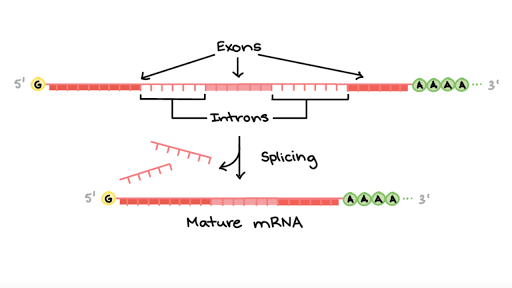
\includegraphics[width=6cm]{../figures/splicing_graphic.png} \caption{} 
\label{fig:splicing}
\end{subfigure}
\begin{subfigure}{.5 \textwidth}
\centering
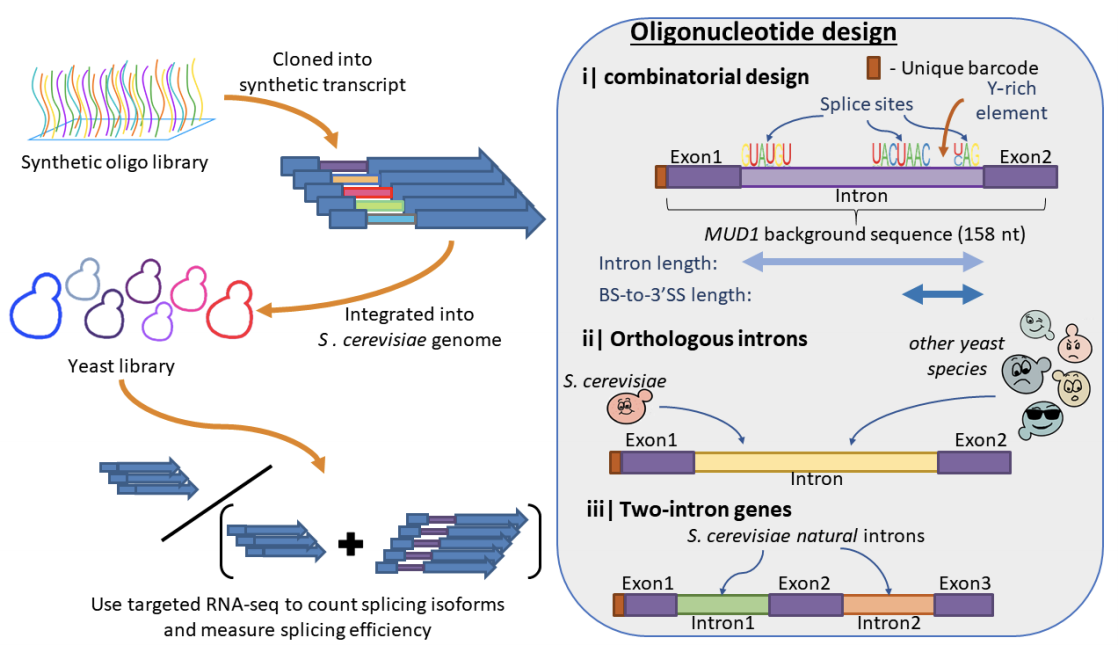
\includegraphics[width=6cm]{../figures/dataset_overview_pilpel.png} \caption{}  
\label{fig:dataset}
\end{subfigure}
\caption{a) mRNA splicing overview. b) Schematic depicting the library of splicing efficiency measurements. Data and figure from Schirman, et al. bioRxiv 2021 \cite{pilpel}.}
\end{figure}
\section{Dataset and Features}
We use the dataset collected by Shirman, et al. \cite{pilpel} of splicing efficiency values for a library of 16268 designed sequence variants in yeast (Figure \ref{fig:dataset}). Each datapoint consists of a sequence of length 1615 nucleotides (A, C, T, or G) along with a corresponding splicing efficiency value (real values from 0 to 1), measured through RNA sequencing. The dataset consists of seven library types with different synthetic sequence design strategies to probe different backgrounds (12376 sequences) and five library types based on naturally occurring intron variants in {\it S. cerevisiae} and other related yeast species (3892 sequences). The sequences were one-hot encoded with a 4-letter vocabulary (A, C, T, or G).
\newline \\
To split the dataset into training, dev, and testing data, we used 90\% of each library type in the training set, and 5\% of each library type in the dev and test sets. By sampling these splits within library types, we ensured that the dev and test set have the same distribution. The original dataset contained the majority (80.3\%) of splicing efficiency values below 0.1; to correct this imbalance, we equalized the data between the ranges $[0, 0.1]$ and $[0.1, 1]$ by resampling. We made sure that near-identical sequences were not shared between the training, dev, and test sets. We explored using different sequence contexts for splicing efficiency predictions: 1. the full 1615 nucleotide mRNA sequence, 2. the intron alone (maximum length 145 nucleotides), or 3. 20 nucleotide windows around three key splicing sequences in the mRNA (120 nucleotides total centered on the {\bf 5' splice site}, {\bf branch site}, and  {\bf 3' splice site} required for splicing \cite{splicingreview}).

\section{ Methods }
\subsection{Baseline Model}
We first tested a baseline model using simple sequence heuristics to assign sequences to a splicing efficiency value. For each sequence in the dev set, we predicted its splicing efficiency value by comparing similarity to wildtype yeast mRNA that have introns that are spliced. If the sequence is not similar to known spliced mRNA's in yeast, we predict a splicing efficiency of 0, and if it is similar, we assign the predicted splicing efficiency value to be  the average splicing efficiency value from the training set (computed using only sequences with splicing level above $\epsilon = 0.001$). \newline \\
To evaluate similarity of sequences in the dev set to wildtype yeast spliced mRNA's we used the following heuristics. At a first approximation, splicing occurs when the cell's splicing machinery recognizes three short key sequences in mRNAs: the 5' splice site (6 nucleotides at the start of an intron), branch site (8 nucleotides in the latter portion of the intron), and 3' splice site (3 nucleotides at the end of the intron) \cite{splicingreview}. First we compute the position weight matrix (nucleotide distribution) for sequence motifs at each of these three key sequences using wildtype yeast mRNAs. We additionally compute two length distributions from wildtype introns: the full length of the intron, and the length between the branch site and 3' splice site. For a tested sequence to be marked as similar to wildtype yeast splicing mRNA's, we require that sequences' score against the position weight matrix and length distributions fall within the 95th percentile of wildtype introns.
\subsection{RNN Model}
LSTM models have been shown to capture long-range base-pairing interactions in RNA sequences \cite{rnn}, which play a role in regulating mRNA splicing efficiency. These long-range interactions represent second-order effects that would not be captured by the baseline model. We implemented a bidirectional LSTM architecture consisting of a first convolutional layer (64 filters, kernel size of 15 and stride-length of 4) followed by a dropout layer, two bidirectional LSTM layers with dropout and batch normalization layers, and a final set of dense layers with ReLU activations.
\subsection{CNN Model}
CNN models have been used fruitfully to predict binary splicing outcomes from mRNA sequence \cite{spliceai}. We trained CNN models with residual blocks to facilitate useful gradient updates, with each residual block including convolution layers, batch normalization layers, and ReLU activations (Figure \ref{fig:architecture}). The final layer of the CNN architectures was a dense layer with a ReLU activation. We explored architectures with varying numbers of residual blocks (one or four), removing add blocks (leaving only convolutional layers), varying the presence of a convolutional layer after the residual block, and varying the amount of sequence context used for prediction. The parameters for filter size, stride length, and number of filters were obtained from the CNN's trained in \cite{spliceai}.
\subsection{Training strategy and evaluation metrics}
Since we are predicting a real-valued outcome, we use a mean-squared error (MSE) regression loss function as implemented in Keras, and we will use a ReLU activation function for the final node in the neural network models. We tuned hyperparameters by evaluating them on the dev dataset, and we evaluate the final models on the test dataset. We trained the RNN and CNN models over 20 epochs using Adam optimization with mini-batches, and we used early stopping for regularization, monitoring the validation loss and ending training after two consecutive epochs with a change in loss of less than 0.001. For each architecture choice, we chose the best of 5 models trained with different random weight initializations. 
\subsection{Implementation} 
All deep learning methods were implemented in Keras using TensorFlow 2.0 \cite{tensorflow}, with logging through wandb and model interpretation through \texttt{tf\_keras\_vis}. Code is available at \texttt{https://github.com/ramyarangan/cs230\_project}.

\section{Experiments and Results}
\subsection{Hyper-parameter exploration}
To decide on hyper-parameters of the network, for the CNN architecture with 4 residual blocks trained on a 120 nucleotide window of sequence data, we varied learning rates (0.01, 0.001, and 0.0001), mini-batch sizes (32, 64, 128), and the momentum parameters (0.9 and 0.95). We found that we were able to achieve the best performance on the validation set for this CNN architecture with a learning rate $\alpha = 0.001$, momentum $\beta_1 = 0.9$, and mini-batch size of 64 within 20 epochs. We additionally chose standard values of $\beta_2 = 0.999$ and a decay value of $0.01$ for Adam optimization. 


\begin{figure}[H]
\centering
\begin{subfigure}{.3 \textwidth}
\centering
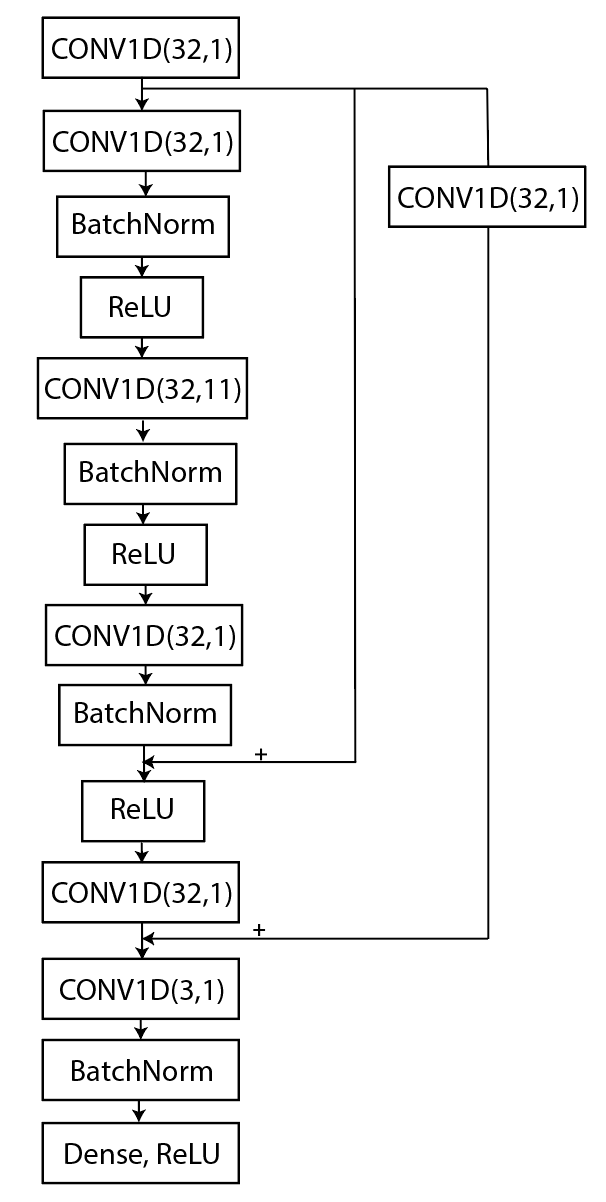
\includegraphics[width=2.5cm]{../figures/cnn_architecture.png} \caption{} 
\label{fig:architecture}
\end{subfigure}
\begin{subfigure}{.65 \textwidth}
\centering
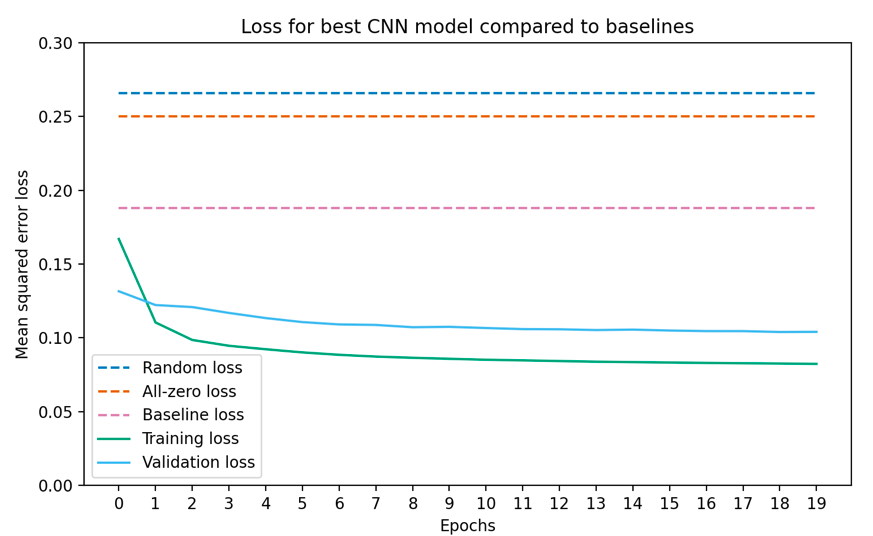
\includegraphics[width=8cm]{../figures/loss.png} \caption{}  
\label{fig:loss}
\end{subfigure}
\caption{Best-performing CNN network. a) CNN architecture for best network. \texttt{CONV(n,f)} layers indicate the number of filters with \texttt{n} and the filter size with \texttt{f}. b) Mean-squared error loss over epochs of training for best network, compared to the baseline model, and models predicting 0 for all examples or random values for all examples.}
\end{figure}

\begin{table}[H]
\centering
\tiny
 \begin{tabular}{||c | c | c | c | c | c | c||} 
 \hline
 Model & Architecture & Sequence context & \# params & Training MSE & Validation MSE & Pearson r \\ [0.5ex] 
 \hline\hline
 Random & Heuristic & Full transcript & 0 & 0.263 & 0.266 & 0 \\ \hline
 Zeros & Heuristic & Full transcript & 0 & 0.250 & 0.258 & nan \\ \hline
 Baseline & Heuristic & Full transcript & 0 & 0.189 & 0.188 & 0.247 \\ \hline
 RNN & 2-layer LSTM & Full transcript & 991329 & 0.251 & 0.258 & nan \\ 
 \hline
 RNN & 2-layer LSTM & 120 nt window & 991329 & 0.251 & 0.258 & nan \\ 
 \hline
 CNN & 4 Residual Blocks & 120 nt window & 57912 & 0.0874 & 0.133 & 0.534 \\ 
 \hline
  {\bf CNN} & {\bf 1 Residual Block + CONV} & {\bf 120 nt window} & {\bf 16536} & {\bf 0.0819} & {\bf0.104 } & {\bf 0.625} \\ 
 \hline
   CNN &1 Residual Block & 120 nt window & 14424 & 0.120 & 0.171 & 0.430 \\ 
 \hline
   CNN & 5 CONV & 120 nt window & 15480 & 0.133 & 0.171 & 0.404 \\
 \hline
   CNN &1 Residual Block + CONV & Full intron & 16536 & 0.117 & 0.134 & 0.506 \\
\hline
   CNN &1 Residual Block + CONV & Full transcript & 16536 & 0.251 & 0.258 & nan\\
 \hline
 \hline
\end{tabular} \newline \\
\caption{Performance of CNN and RNN architectures on predicting splicing efficiency. Training and validation mean-squared errors (MSE) are reported. The Pearson r is reported for the dev set for each architecture, and is reported as nan in cases where the model predicts only 0 values. The best model is bolded.}
\label{tab:perf}
\end{table}

\subsection{Model performance} 
When the baseline model is used to predict splicing efficiency values for the development set, the mean-squared error loss on the dev set is 0.188 compared to the mean-squared error loss of 0.266 for a random model that predicts uniform random values from 0 to 1 for all dev set examples, or 0.258 for a model that predicts 0 for all examples. The LSTM architectures were not able to improve loss beyond the a network that predicts all zero values. However, most CNN architectures tested decreased mean-squared error loss over training epochs, leading to lower MSE values on the training and validation data and higher Pearson r correlation values to the validation data (Table \ref{tab:perf}). The best architecture included one residual block and additional convolutions followed by a dense layer (Figure \ref{fig:architecture}), with both training and validation mean-squared error loss falling below that of the baseline model (Figure \ref{fig:loss}). The MSE on the test set for this best architecture was 0.102 (similar to validation MSE), compared to 0.202 MSE on the test set for the baseline model. \newline \\
Including a residual block improved training, achieving better MSE and Pearson R correlation to the validation data (compare 1 Residual Block + CONV model with 0.104 validation MSE to the 5 CONV model that contains no Add layers with 0.171 validation MSE). However, adding additional residual blocks (compare the 4 Residual Blocks model with 0.133 validation MSE to the 1 Residual Block + CONV model with 0.104 validation MSE). The best models made predictions using windows of size 40 centered on three key splicing sequences (120 nucleotides total) (Table \ref{tab:perf}). While models given the full-length transcript were not able to perform better than a network predicting all zero values, a model using the full intron was able to achieve good performance with validation MSE 0.134 (Table \ref{tab:perf}). This indicates that the precise locations of key splicing sequences are not necessary inputs for deep learning approaches predicting splicing efficiency. 

\subsection{Error analysis and interpretation}
We proceeded to analyze the best CNN architecture depicted in Figure \ref{fig:architecture}. We observed that the distribution of splicing efficiency values predicted by the network was close to the distribution of the validation set, with many constructs having 0 splicing efficiency. We analyzed the mean-squared error for each library subtype. We found close to 0 mean-squared error for the control library designs, which consisted of five libraries and 3219 sequences intended to splice poorly; the splicing efficiency values for constructs in these sets were nearly all 0. We also saw better than random performance on most other library types. However, performance on the orthologous sequence library (introns naturally occurring in species related to {\it S. cerevisiae}) was poor, perhaps due to the limited number (961) of training examples in this set. To interpret the features of input sequences that were used for predictions, we used SmoothGrad \cite{smoothgrad}, producing saliency maps as shown in Figure \ref{fig:saliency}. These maps suggest that the random library barcode region (positions 8-14) is correctly not used for splicing prediction, and that the branch site (positions 60-67) has high saliency for prediction. However, interestingly, the full sequence window is used by the CNN to make predictions, compared to the baseline model which uses only regions indicated as "canonical splicing sequences" in Figure \ref{fig:saliency}.

\begin{figure}[H]
\centering
%\begin{subfigure}{0.3\textwidth}
%\begin{subfigure}{\textwidth}
%\centering
%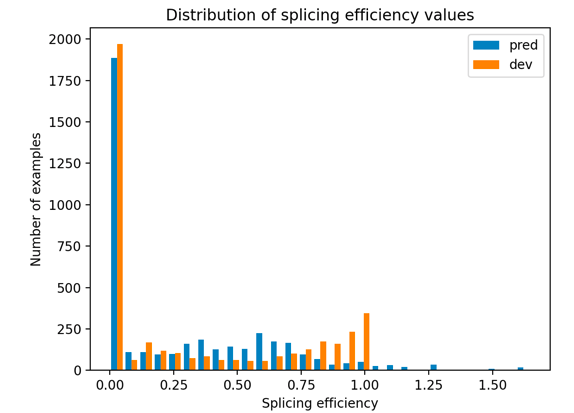
\includegraphics[width=\textwidth]{../figures/distribution.png} \caption{}
%\label{fig:distribution}
%\end{subfigure} \\
\begin{subfigure}{0.3\textwidth}
\centering
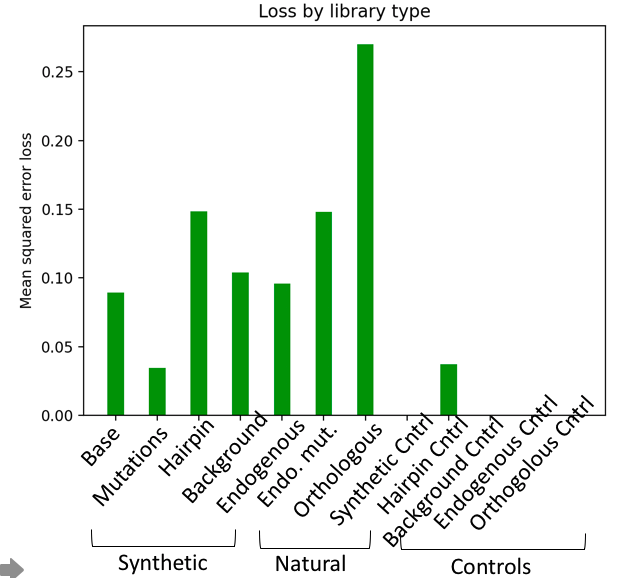
\includegraphics[width=0.95\textwidth]{../figures/library_type.png} \caption{} 
\label{fig:library}
\end{subfigure}%
%\end{subfigure}%
\begin{subfigure}{0.7\textwidth}
\centering
 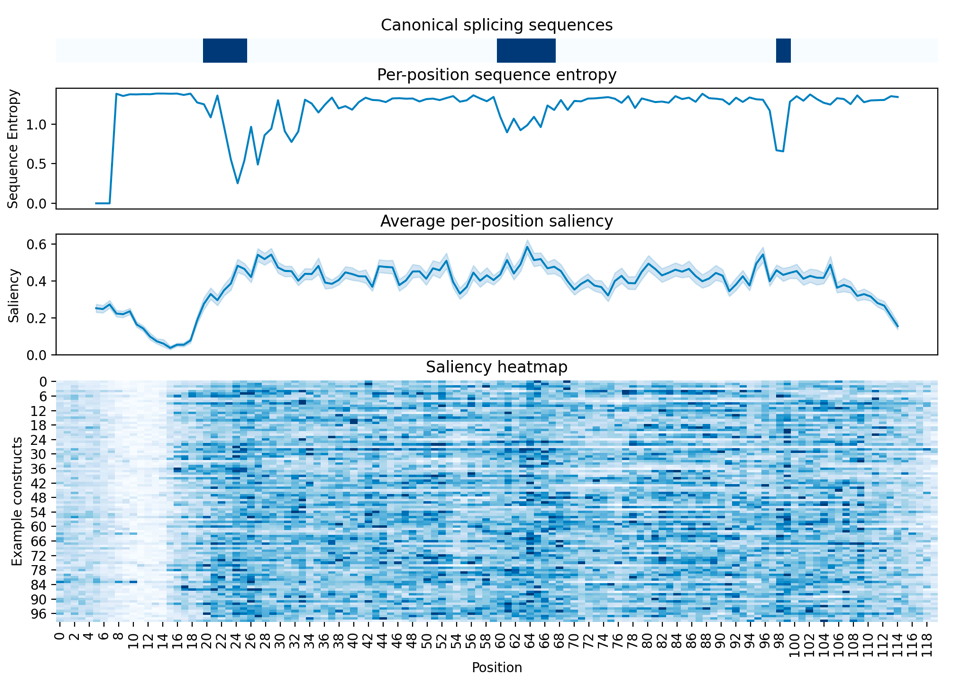
\includegraphics[width=0.75\textwidth]{../figures/saliency.png} \caption{} 
\label{fig:saliency}
\end{subfigure}
\caption{Error analysis and interpretation for best CNN network. a) Mean-squared error loss for each library. b) Saliency of each position of the sequence window for the final prediction. Per-position sequence entropy indicates sequence variation in the training dataset, and canonical splicing sequences indicate positions used by the baseline model.}
\end{figure}

\subsection{Discussion} 
The CNN architectures tested were able to extract additional information from a broader sequence context than the baseline model, producing predictions with lower mean-squared error and higher Pearson correlation to measured splicing efficiency values. With fewer than 100,000 sequences for training, the best-performing architectures had relatively few parameters, with shallower CNN architectures outperforming deeper CNN's or LSTM models. This contrasts with SpliceAI \cite{spliceai} which trained a much deeper CNN using a larger training dataset on a similar prediction task. In all models performing better than random, some variance remains, with training MSE below validation MSE, suggesting that approaches to reduce overfitting may prove useful in this setting. We used early stopping during training, and could further add dropout regularization to the CNN architectures to further reduce overfitting. 

\section{Conclusion and Future Work }
Here we found that relatively simple CNN architectures were able to learn splicing efficiency values better than baseline approaches using conventional knowledge for evaluating splicing sequences. Simpler CNN architectures were better performing than LSTM models and deeper CNN's with more parameters. In the future, it will be important to evaluate how robustly the predictions from this network generalize, perhaps using clustering to better separate training and validation data, augmenting with datasets from orthogonal studies, and ultimately, making predictive tests that can be assessed with additional sequencing experiments.

\section{Contributions}
Ramya performed all modeling and analysis for this project. Huizi Mao provided advice as a Project TA. 


\begin{thebibliography}{9}
\bibitem{pilpel} 
Schirman, D., Yakhini, Z., Dahan, O., Pilpel, Y.
\textit{Sequence determinants and evolution of constitutive and alternative splicing in yeast species}. 2021. bioRxiv. 

\bibitem{seelig} 
Rosenberg, A.B., Patwardhan, R.P., Shendure, J., Seelig, G.
\textit{Learning the sequence determinants of alternative splicing from millions of random sequences.}. 2015. Cell, 163 (698-711). 

\bibitem{spanr}
Xiong, H.Y., Alipanahi, B., Lee, L.J., et al. 
\textit{The human splicing code reveals new insights into the genetic determinants of disease.} 2015. Science, 347 (1254806).

\bibitem{spliceai} 
Jaganathan, K., Panagiotopoulou, S. K., McRae, J.F., et al. 
\textit{Predicting splicing from primary Sequence with deep learning}. 2019. Cell, 176 (535-548). 

\bibitem{rnn} 
Wu, M., Andreasson, J.O.L, Kladwang, W., et al. \textit{Prospects for recurrent neural network models to learn RNA
biophysics from high-throughput data}. 2018. bioRxiv.

\bibitem{splicingreview}
Wilkinson, M.E., Charenton, C., Nagai, K. \textit{RNA Splicing by the Spliceosome}. 2019. Annual Review of Biochemistry, 89 (359-388).

\bibitem{tensorflow}
Abadi, M., Agarwal, A., Barham, P., et al. \textit{TensorFlow: Large-Scale Machine Learning on Heterogeneous Distributed Systems}. 2016. bioRxiv.

\bibitem{smoothgrad}
Smilkov, D., Thorat, N., Kim, B., Viegas, F., Wattenberg, M. \textit{SmoothGrad: removing noise by adding noise}. 2017. arXiv.
\end{thebibliography}


\end{document}